\chapter{Design And Implementation}

\section{Overall Design}
\par
Sign Language recogniser is developed with Inception V3 model which is a convolutional neural network.\\

This model was known to classify an image across 1000 categories supplied by the ImageNet academic competition with an error rate that approached human performance. As sign language is a multi classification problem it needs a highly designed model which will be able to differentiate even small differences in hand gestures. 

\begin{figure}[H]
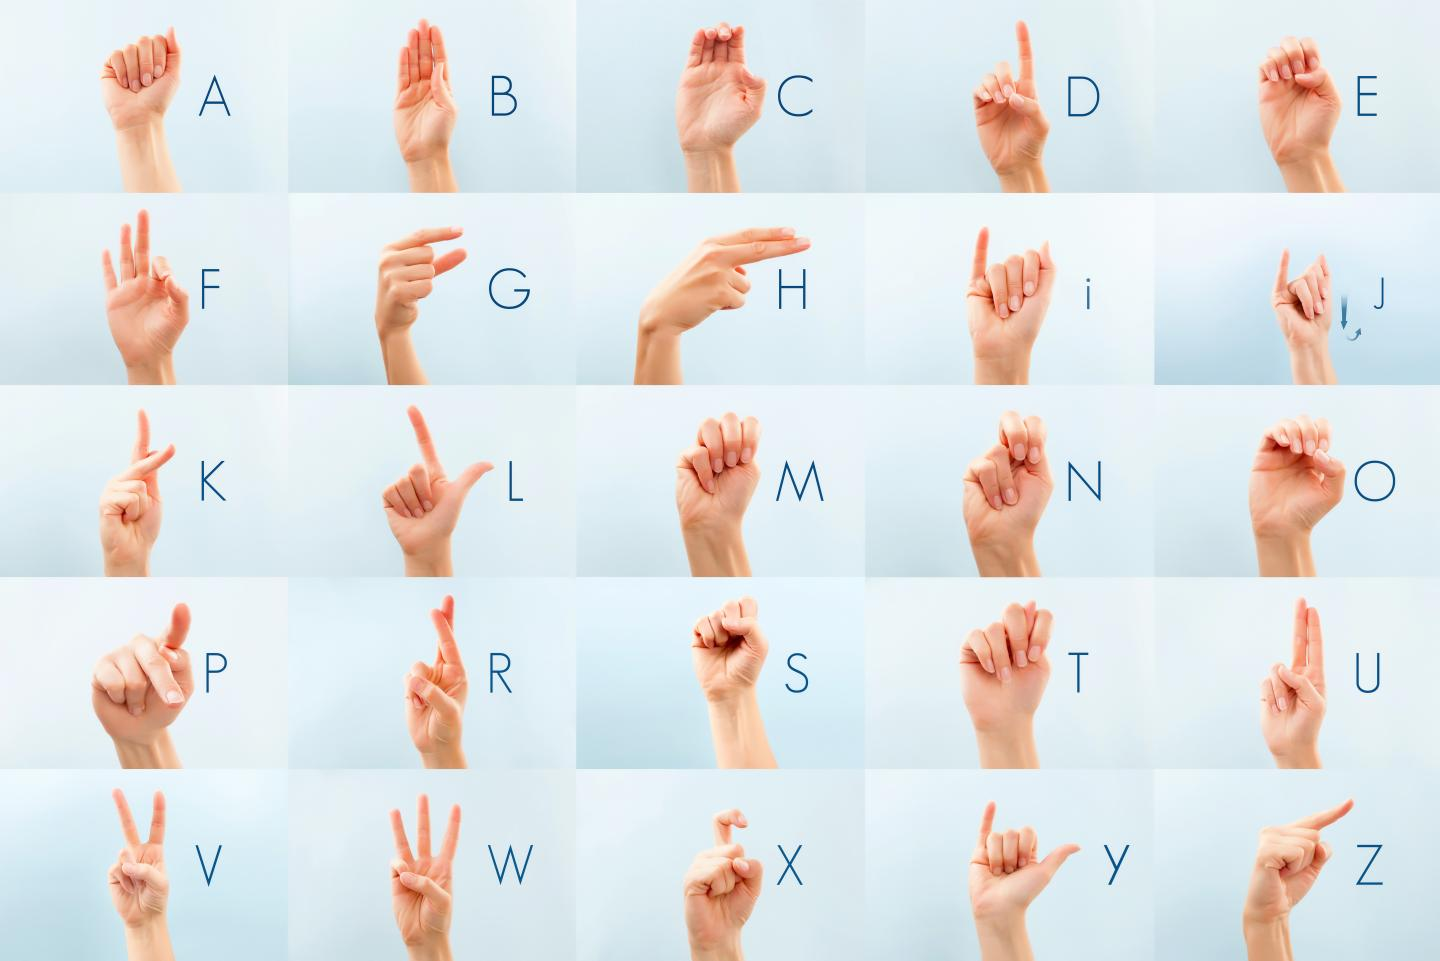
\includegraphics[scale=0.3]{report/hand.jpg}}
\caption{American Sign language}
\end{figure}

\section{User Interfaces}
The UI is designed with Tkinter.
Tkinter is a Python binding to the Tk GUI toolkit. It is the standard Python interface to the Tk GUI toolkit, and is Python's de facto standard GUI. Tkinter widgets such as button, label etc are used here for designing a simple UI which connects the whole project code into a single entity. 

\section{Technology Stack}
\subsection {Deep Learning} Deep learning is a sub-field of machine learning dealing with algorithms inspired by the structure and function of the brain called artificial neural networks. In other words, It mirrors the functioning of our brains. Deep learning algorithms are similar to how nervous system structured where each neuron connected each other and passing information. Deep learning models work in layers and a typical model atleast have three layers. Each layer accepts the information from previous and pass it on to the next one.

\subsection{Tensorflow}Tensorflow is a computational framework for building machine learning models. TensorFlow provides a variety of different toolkits that allow us to construct models at our preferred level of
abstraction. It is possible to use lower-level APIs to build models by defining a series of mathematical operations.
\subsection{OpenCV} OpenCV is an open source C++ library for image
processing and computer vision, originally developed by Intel and now
supported by Willow Garage. Therefore it is not mandatory for your
OpenCV applications to be open or free. It is a library of many inbuilt
functions mainly aimed at real time image processing.

\section{Methodology}
The program applies Transfer Learning to this existing model and re-trains it to classify a new set of images.

\subsection{Transfer Learning}
Modern image recognition models have millions of parameters. Training
them from scratch requires a lot of labeled training data and a lot of
computing power (hundreds of GPU-hours or more). Transfer learning is a
technique that shortcuts much of this by taking a piece of a model that has
already been trained on a related task and reusing it in a new model.

\subsection{Bottlenecks} The script can take thirty minutes or more to complete, depending on the
speed of your machine. The first phase analyzes all the images on disk and
calculates and caches the bottleneck values for each of them. 'Bottleneck'
is an informal term we often use for the layer just before the final output
layer that actually does the classification. (TensorFlow Hub calls this an
"image feature vector".) This penultimate layer has been trained to output
a set of values that's good enough for the classifier to use to distinguish
between all the classes it's been asked to recognize. That means it has to be
a meaningful and compact summary of the images, since it has to contain
enough information for the classifier to make a good choice in a very small
set of values. The reason our final layer retraining can work on new classes
is that it turns out the kind of information needed to distinguish between
all the 1,000 classes in ImageNet is often also useful to distinguish between
new kinds of objects.
\begin{figure}[H]
\centering
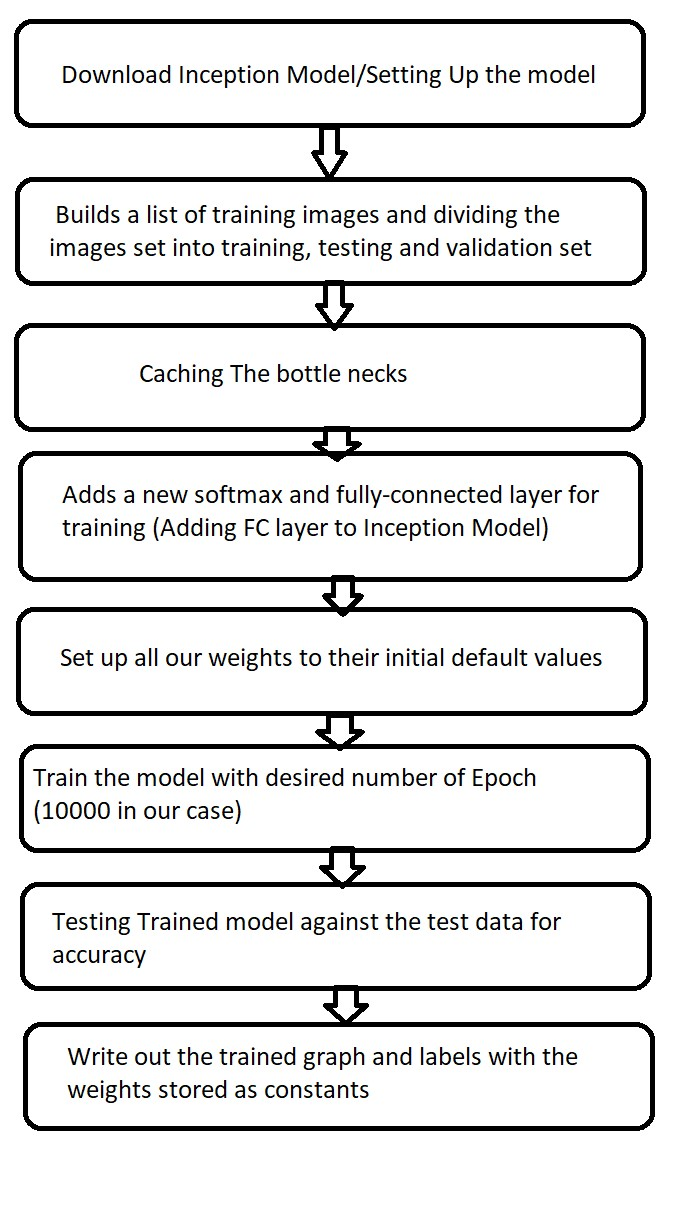
\includegraphics[scale=0.4]{one}
\caption{Algorithm}
\end{figure}

\subsection{Training} Once the bottlenecks are complete, the actual training of the top layer of
the network begins. You'll see a series of step outputs, each one showing
training accuracy, validation accuracy, and the cross entropy. The training
accuracy shows what percent of the images used in the current training
batch were labeled with the correct class. The validation accuracy is the
precision on a randomly-selected group of images from a different set. The
key difference is that the training accuracy is based on images that the
network has been able to learn from so the network can overfit to the noise
in the training data. A true measure of the performance of the network is to
measure its performance on a data set not contained in the training data --
this is measured by the validation accuracy. If the train accuracy is high
but the validation accuracy remains low, that means the network is
overfitting and memorizing particular features in the training images that
aren't helpful more generally. Cross entropy is a loss function which gives
a glimpse into how well the learning process is progressing. The training's
objective is to make the loss as small as possible, so you can tell if thelearning is working by keeping an eye on whether the loss keeps trending
downwards, ignoring the short-term noise.

\section{System Design}
\par
The system is designed with inception v3 model. The model is retrained to create an efficient system for sign language. In the retraining phase, all the parameters are passed as arguments to the system.

% debug: include image

\subsection{Inception V3 Model}
\par
Inception v3 is a widely-used image recognition model that has been shown to attain greater than 78.1\% accuracy on the ImageNet dataset. The model is the culmination of many ideas developed by multiple researchers over the years.
The model itself is made up of symmetric and asymmetric building blocks, including convolutions, average pooling, max pooling, concats, dropouts, and fully connected layers. Batchnorm is used extensively throughout the model and applied to activation inputs. Loss is computed via Softmax.
\begin{figure}[H]
\centering
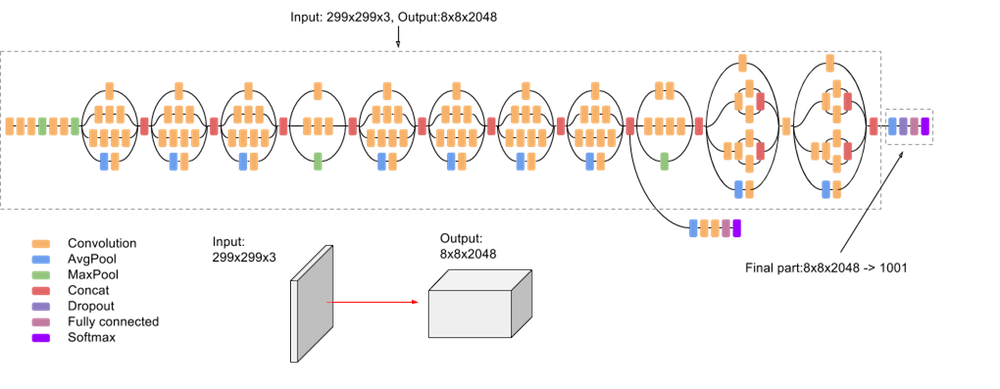
\includegraphics[scale=0.46]{two}
\caption{Inception V3 Architecture}
\end{figure}



\subsection{Recognition using image as input}
\par
It purely uses the concept of deep learning pattern recognition. When a new images is supplied the features of the image is extracted and it is compared with the features extracted from training dataset. The prediction is displayed with confidence score for each character.

\subsection{Recognition from live video}
\par
Image processing and deep learning are used here for the recognition purpose. With the help of OpenCV images are captured from video and this image processed to identify the sign language character. Words can be build with the help of each character by character video understanding. 

\subsection{Screenshots}


\begin{figure}[H]
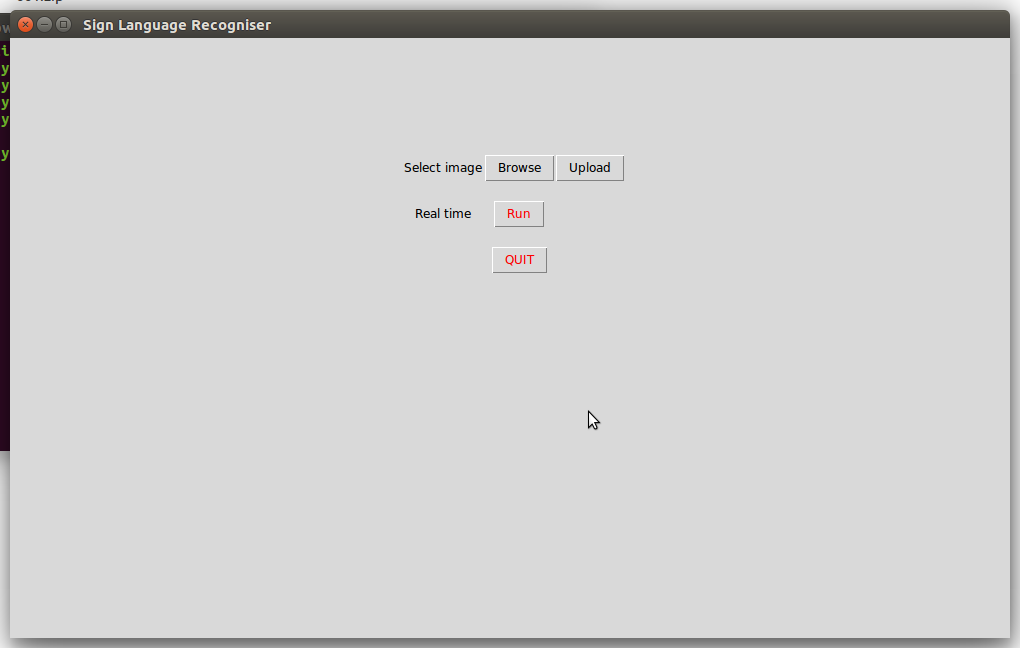
\includegraphics[scale=0.4]{ss1}
\caption{GUI}
\end{figure}

\begin{figure}[H]
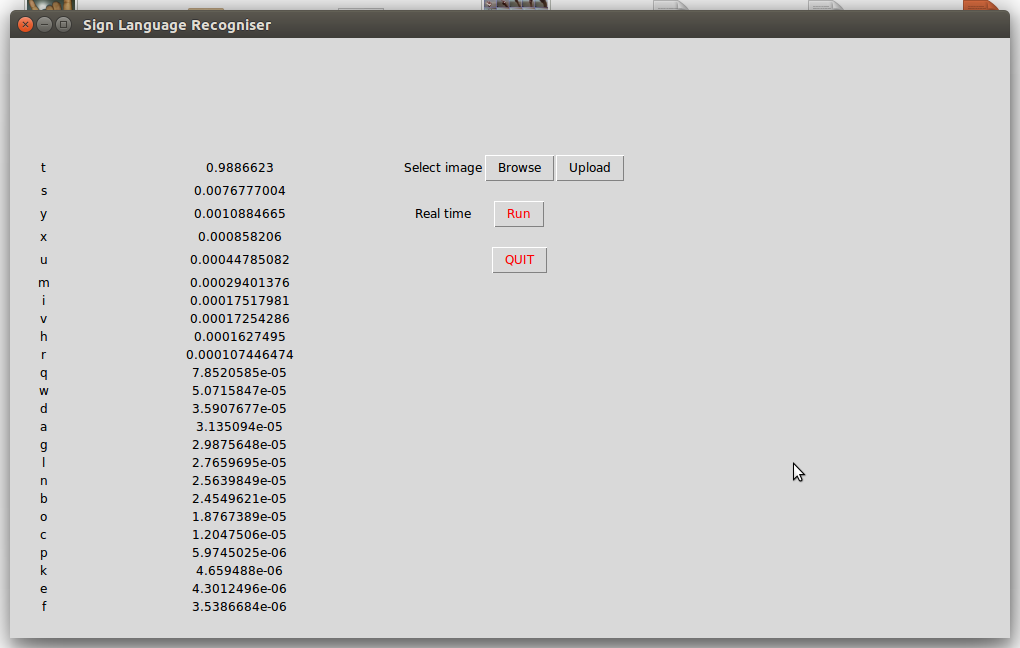
\includegraphics[scale=0.4]{ss2}
\caption{Prediction after uploading image}
\end{figure}


\begin{figure}[H]
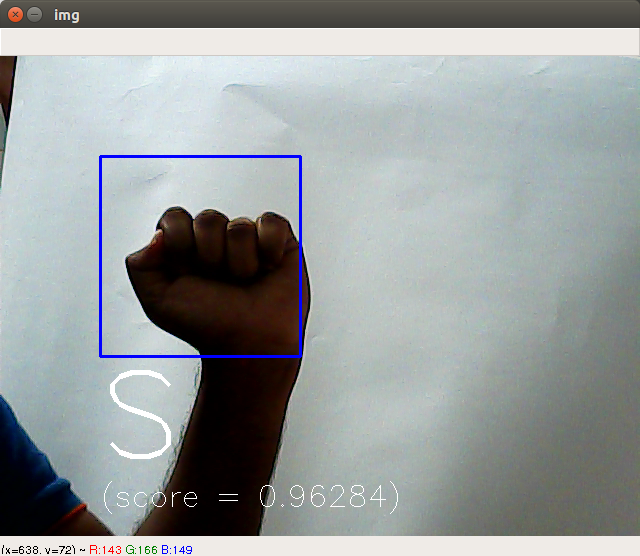
\includegraphics[scale=0.5]{ss3}
\caption{Sign recognition from live video}
\end{figure}


